\documentclass[10pt,aspectratio=169]{beamer}

\usepackage[utf8]{inputenc}
\usepackage{physics}
\usepackage{siunitx}
\usepackage{tcolorbox}
\usetheme{Berkeley}
\usecolortheme{spruce}

%font
\usepackage{lmodern}% http://ctan.org/pkg/lm

% for degree symbol
\usepackage{textcomp}

% compile only one certain frame
%\includeonlyframes{1}

\usepackage{tikz}
\usetikzlibrary{arrows.meta,shapes.arrows}
%\usetikzlibrary{external}
%\tikzexternalize

\tikzset{
  every overlay node/.style={
    draw=black,fill=white,rounded corners,anchor=north west,
  },
}
% Usage:
% \tikzoverlay at (-1cm,-5cm) {content};
% or
% \tikzoverlay[text width=5cm] at (-1cm,-5cm) {content};
\def\tikzoverlay{%
   \tikz[baseline,overlay]\node[every overlay node]
}%

% for strikethrough
\usepackage{ulem}

% Some font sizes and other parameters
\setbeamerfont{title in sidebar}{size=\fontsize{4.5pt}{4.5pt}}
\setbeamerfont{author in sidebar}{size=\fontsize{4.5pt}{4.5pt}}
\setbeamerfont{section in sidebar}{size=\fontsize{4pt}{4pt}}
\setbeamerfont{subsection in sidebar}{size=\fontsize{3.5pt}{3.5pt}}
\setbeamerfont{subsection in toc}{size=\scriptsize}
\setcounter{tocdepth}{1}

%\AtBeginSection[]
%{
%        \begin{frame}<beamer>
%        \tableofcontents[currentsection]
%        \end{frame}
%}

\graphicspath{{../images/}}

%Information to be included in the title page:
\title{Atmospheric Effects in Ground-Based Observations of the Cosmic
Microwave Background}
\subtitle{The Case of the LSPE/Strip Telescope}
\author[Matteo Savatteri]{Matteo Savatteri\\[1ex]  {\footnotesize Supervisor:
Aniello Mennella\\[1ex]  Co-supervisor: Stefano Mandelli}}
\institute{Università degli Studi di Milano} \date{July 6, 2021}

\begin{document}

\frame{\titlepage}

\section*{Outline}
\begin{frame}
\frametitle{Table of Contents}
\tableofcontents
\end{frame}

\section{An Introduction to the CMB Radiation}

\begin{frame}
\frametitle{The Cosmic Microwave Background}

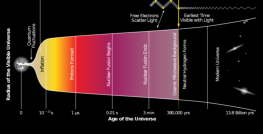
\includegraphics[width=0.63\textwidth]{universe_expansion_2}
\pause
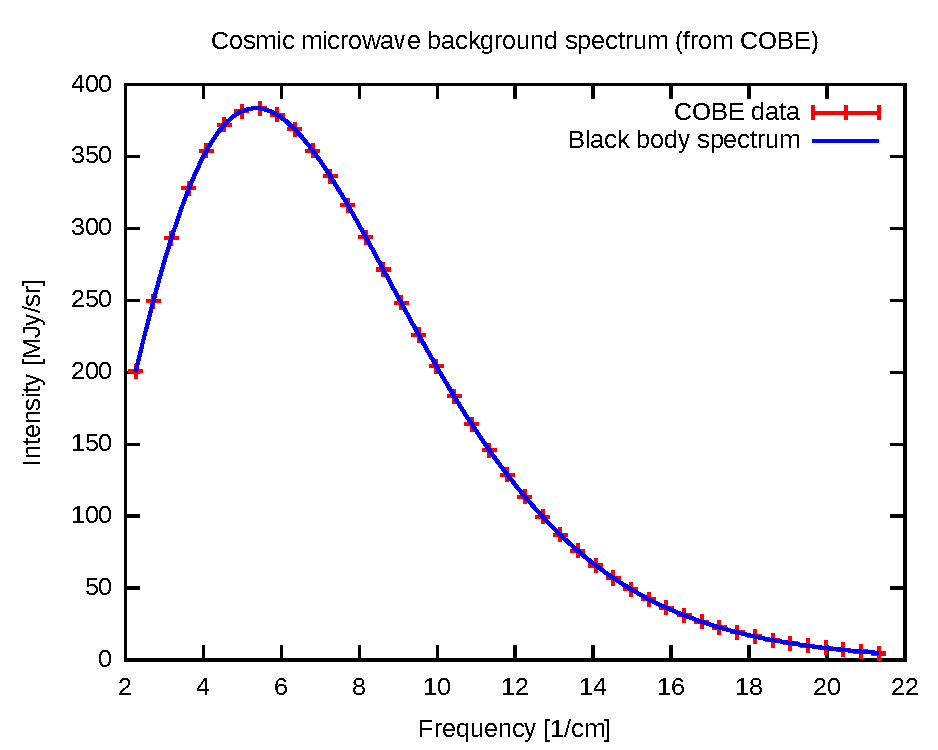
\includegraphics[width=0.35\textwidth]{CMB_Spectrum_COBE}

\pause

\vspace{0.5cm}
\hfill Universe expansion $\rightarrow$ \alert{$\sim 2.73 K$}

\end{frame}

\subsection{Temperature Anisotropies}

\begin{frame}
\frametitle{Intensity Anisotropies}

\begin{columns}
        \begin{column}{0.65\textwidth}
                \centering
                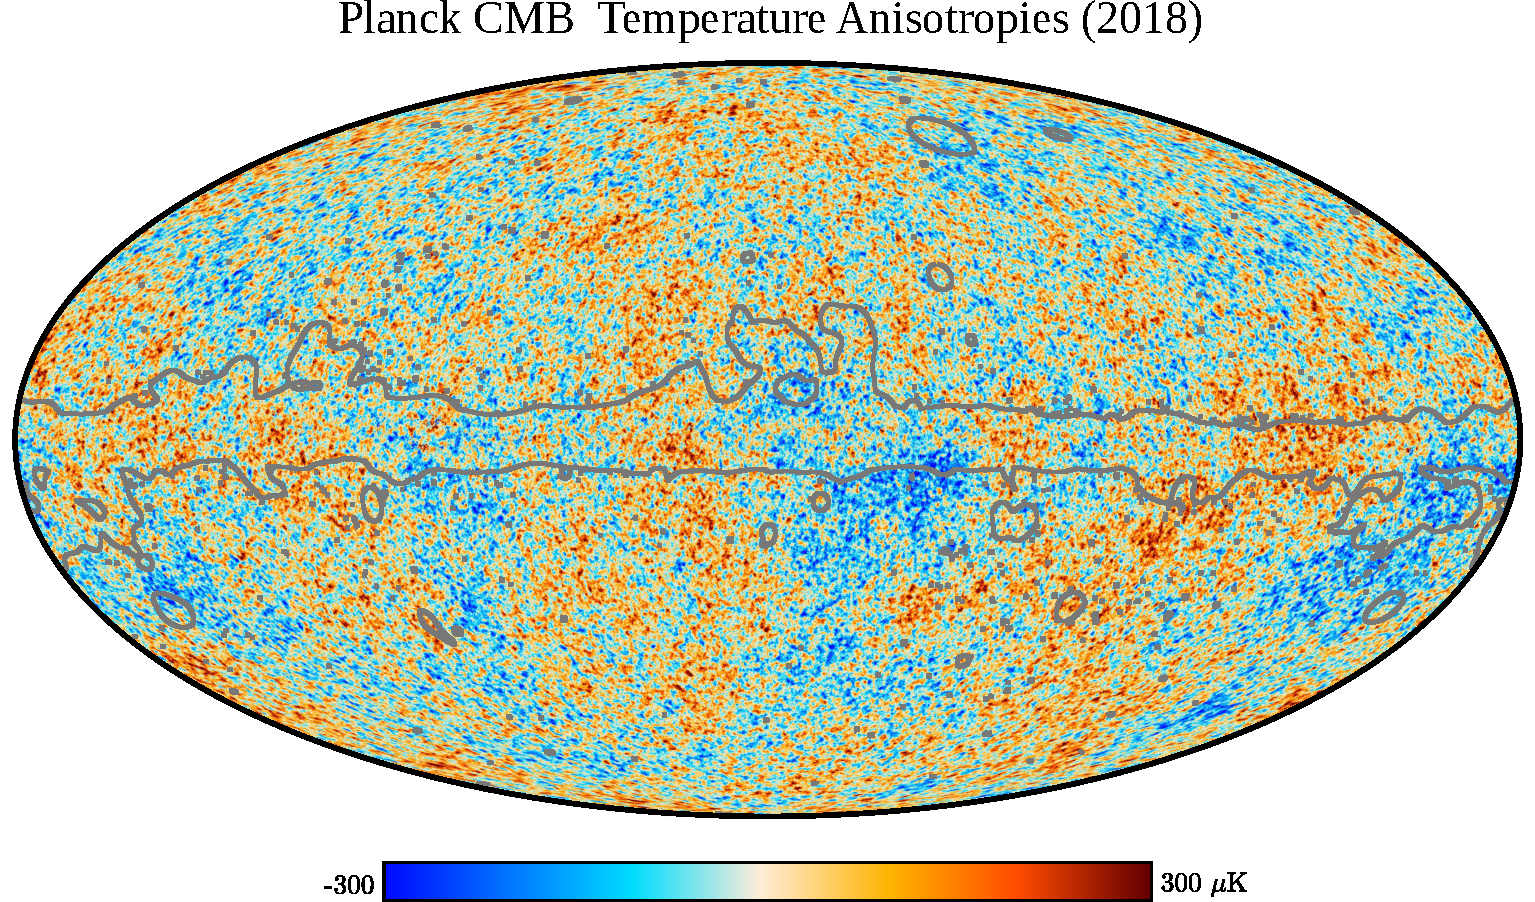
\includegraphics[width=1\textwidth]{Planck_2018_T_CMB_small}
        \end{column}
        \pause
        \begin{column}{0.33\textwidth}
        \scriptsize
                \begin{block}{Temperature Power Spectra ($C_l$)}
                        \scriptsize
                        \begin{align}
                                \frac{\var{T\qty(\theta,\phi)}}{\bar T} & =
                                \sum^\infty_{l=0}\sum^l_{m=-l} a_{l,m}
                                Y_{l,m}\qty(\theta,\phi) \\
                                \textcolor{red}{C_l} & = \frac{1}{2l + 1}
                                \sum_m \expval{a_{l,m} a^*_{l',m'}}
                        \end{align}
                \end{block}
                \pause
                \centering
                \Large $\downarrow$\\
                \normalsize
                \textcolor{red}{Density contrast in primordial plasma}
        \end{column}
\end{columns}

\end{frame}

\subsection{CMB Polarization}

\begin{frame}
\frametitle{CMB Polarization}

\begin{columns}
        \begin{column}{0.38\textwidth}
                \centering
                \large \alert{CMB photons\\
                $\downarrow$\\
                 Thomson scattering events
                during recombination}
        \end{column}

        \pause

        \begin{column}{0.10\textwidth}
                \centering
                \huge $\rightarrow$
        \end{column}

        \begin{column}{0.45\textwidth}
                \centering
                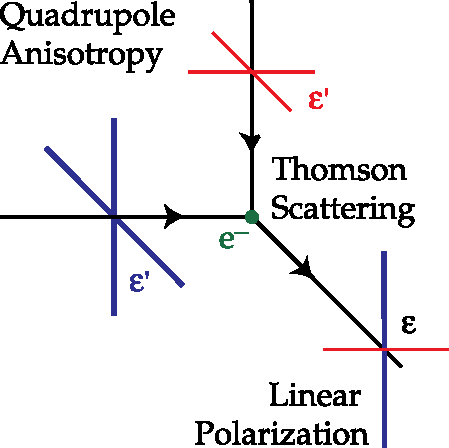
\includegraphics[width=\textwidth]{thomson_scattering}
        \end{column}
\end{columns}

\end{frame}

\begin{frame}
\frametitle{Polarization Anisotropies}

\begin{columns}
        \begin{column}{0.60\textwidth}
                \centering
                \only<1-2>{
                        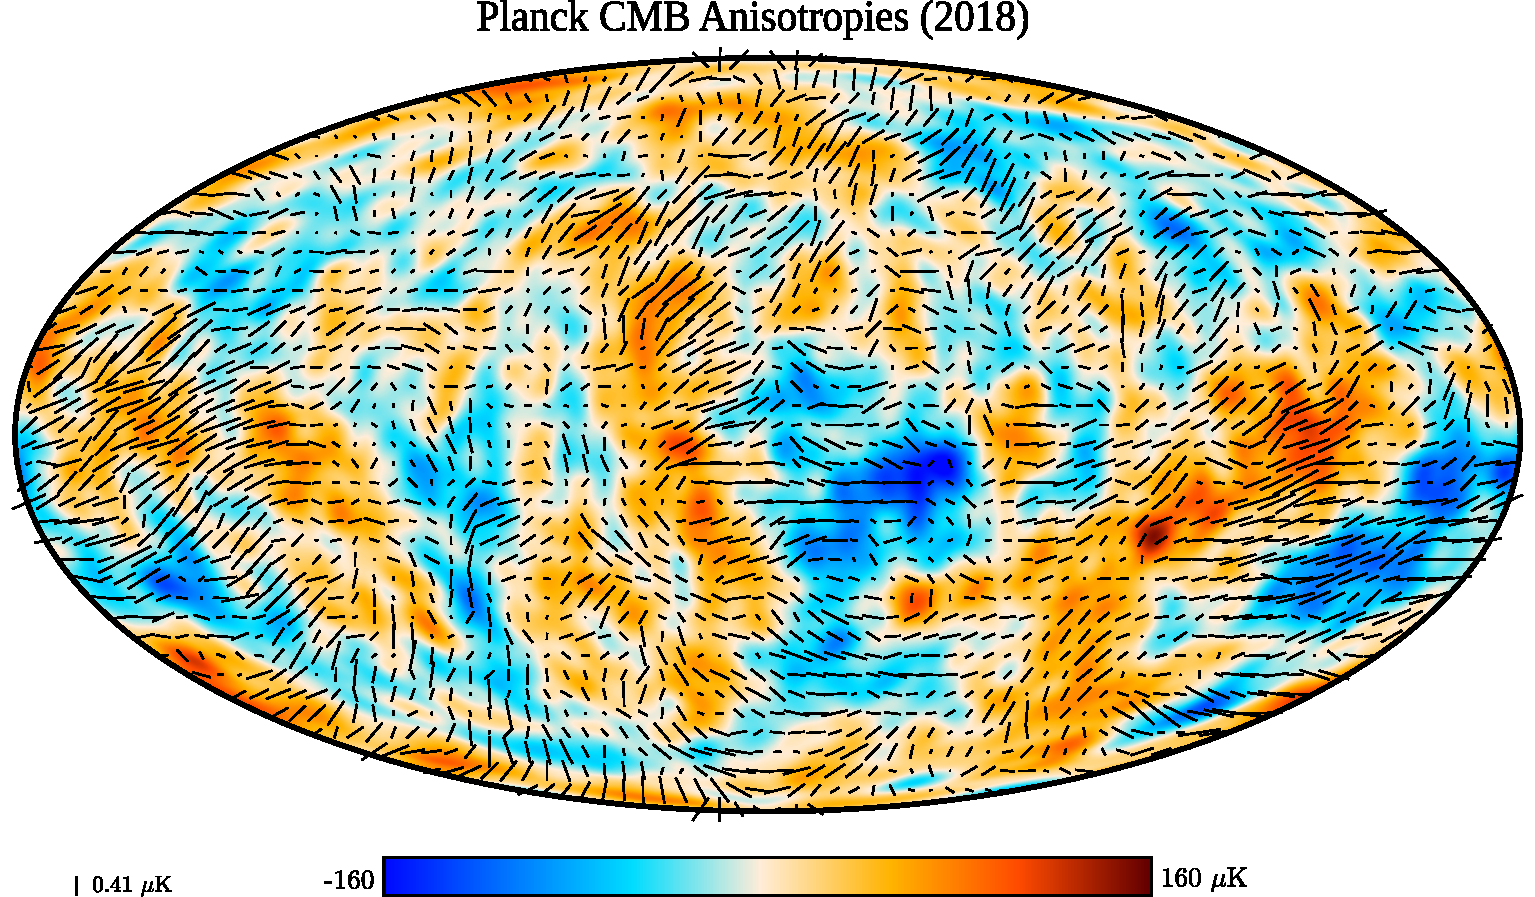
\includegraphics[width=1\textwidth]{Planck_2018_Pol_CMB}
                }
                \only<3>{
                        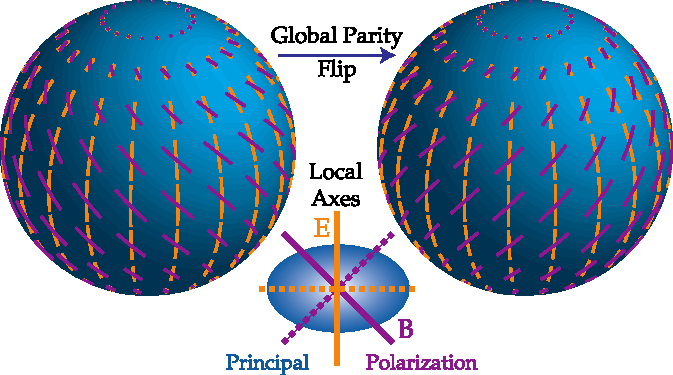
\includegraphics[width=1\textwidth]{eb_modes_patterns}
                }
        \end{column}
        \pause
        \begin{column}{0.38\textwidth}
        \scriptsize
                \begin{block}{Polarization Anisotropies}
                        \tiny
                        \begin{equation}
                                (Q \pm iU)\qty(\theta,\phi) =
                                \sum^\infty_{l=0}\sum^l_{m=-l}
                                a^{\qty(\pm 2)}_{l,m}
                                Y^{\qty(\pm 2)}_{l,m}\qty(\theta,\phi)
                        \end{equation}
                \end{block}
                \pause
                \begin{tcolorbox}
                        Linear combinations:\\
                        \large \alert{E-} and \alert{B-modes}
                \end{tcolorbox}
        \end{column}
\end{columns}

\end{frame}

\section{The B-modes Detection Challenge}

\begin{frame}
\frametitle{PGW B-modes}

\begin{columns}
        \begin{column}{0.58\textwidth}
                \centering
                \alert{State of the art \& prediction:}\\
                \includegraphics<1>[width=1.15\textwidth]{CMB-S4_polarization_status}
                \includegraphics<2->[width=1.15\textwidth]{CMB-S4_polarization_status_b_modes}
                \vspace{0.25cm}
        \end{column}
                \onslide<3>{
                \begin{column}{0.35\textwidth}
                        \centering
                        \begin{tcolorbox}
                                \small
                                B-Modes $\rightarrow$\\
                                \centering
                                \alert{Primdordial Gravitational Waves}
                                \tcblower
                                \centering
                                \large \textcolor{red}{Smoking Gun\\Inflation!}
                        \end{tcolorbox}
                        \huge $\downarrow$\\
                        \large
                        \textcolor{red}{Solves some Big Bang problems}
                \end{column}
                }
\end{columns}

\end{frame}

\subsection{LSPE/Strip}

\begin{frame}
\frametitle{LSPE/Strip}

\begin{columns}
        \begin{column}{0.38\textwidth}
                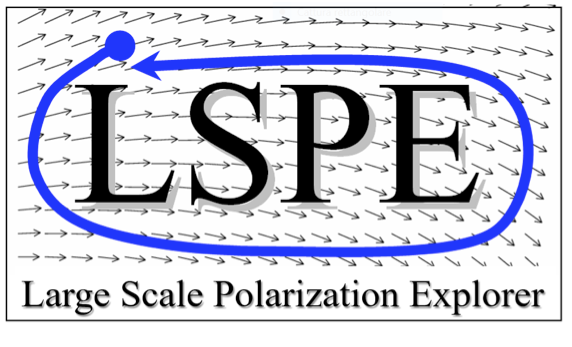
\includegraphics[width=0.30\textwidth]{lspe}
                
\includegraphics[width=0.31\textwidth]{Logo-ASI-2019}
                
\includegraphics[width=0.31\textwidth]{Logo_INFN}
                \begin{itemize}
                        \item<2-> \alert{Upper limit} to B-modes intensity
                        \item<3-> \alert{SWIPE} $\rightarrow$
                        balloon-borne, \SIrange{140}{240}{\giga\hertz}
                        \item<4-> \alert{Strip} $\rightarrow$ Observatorio del
                        Teide
                \end{itemize}
                \onslide<5->{
                        \begin{tcolorbox}[title=Focal Plane $\rightarrow$
                        polarimeters, top=1pt,
                        bottom=1pt]
                                \alert{\SI{43}{\giga\hertz}} (Q-band)
                                \tcblower
                                \alert{\SI{95}{\giga\hertz}} (W-band)
                        \end{tcolorbox}
                }
        \end{column}
        \onslide<4->{
                \begin{column}{0.58\textwidth}
                        \includegraphics<4>[width=1\textwidth]{observatorio_teide}
                        \includegraphics<5>[width=1\textwidth]{strip-focal-plane_2}
                \end{column}
        }
\end{columns}

\end{frame}

\subsection{Atmospheric Effects in CMB Observations}

\begin{frame}
\frametitle{Atmospheric Effects in CMB Observations}

\begin{columns}
        \begin{column}{0.35\textwidth}
                \centering
                \normalsize Atmospheric emission:
                \small
                \begin{itemize}
                        \item<2-> Almost \alert{unpolarized} \large
                        \onslide<3->{\textcolor{red}{but}\dots}
                        \item<3-> Increases \alert{optical loading}
                        $\rightarrow$\\  $>$ \alert{white noise}
                        \item<4-> $H_2 O$ \alert{Turbulent} structure
                \end{itemize}
                \onslide<5->{
                        \huge $\downarrow$
                        \begin{tcolorbox}
                                \centering
                                \small
                                Temporal \& spatial
                                \large \textcolor{red}{correlation}
                                \small in detected signal
                        \end{tcolorbox}
                }
        \end{column}
        \begin{column}{0.63\textwidth}
                \includegraphics<5>[width=1\textwidth]{clouds}
        \end{column}
\end{columns}

\end{frame}

\section{The Atmopsheric Emission Model}

\subsection{Atmospheric Radiative Transfer}

\begin{frame}
\frametitle{Atmospheric Radiative Transfer}

\begin{itemize}
\item<1-3,5-> Atmosphere $\rightarrow$ \alert{dispersive} medium $\rightarrow \epsilon = \epsilon_R + i\epsilon_I$
\item<2-3,5-> $\epsilon_R \propto \sqrt{n_\nu}$,
          \quad $\epsilon_I \propto \alpha_\nu$ \onslide<3->{$\rightarrow$  $O_2$, $H_2O$}
\end{itemize}

\only<4>{
\begin{tikzpicture}[remember picture,overlay]
\node at (6,-1.8) {\includegraphics[width=0.70\textwidth]{transmittance_teide}};
\end{tikzpicture}
}

\begin{block}{Radiative Transfer Equation}<5->
\begin{equation}
\frac{dI_\nu}{ds} = -\alpha_\nu I_\nu + j_\nu
\end{equation}
\end{block}

\begin{block}{Atmospheric Brightness Temperature}<6->%
\begin{equation}
\textcolor{red}{T_{atm}(\nu)} = T_{sky}(\nu) - T_{CMB}(\nu)e^{-\tau_A(\nu)}%
\onslide<7>{\rightarrow \textit{\alert{CMB Atmospheric Library}}}%
\end{equation}%
\end{block}%

\end{frame}

\subsection{ECMWF ERA5 Atmospheric Reanalisys}

\begin{frame}
\frametitle{ECMWF ERA5 Atmospheric Reanalisys}

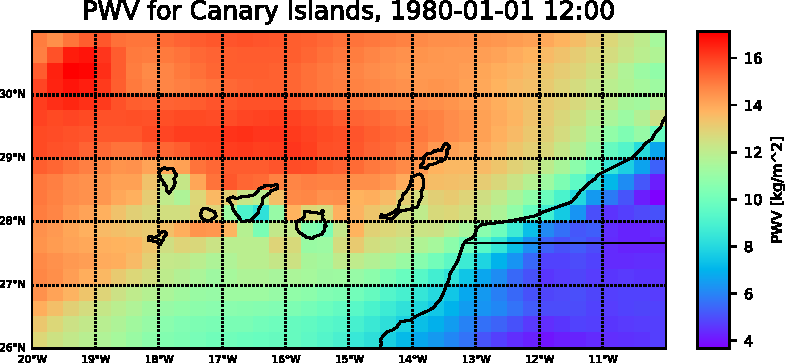
\includegraphics[width=1\textwidth]{PWV_Canary_Islands_1980-01-01_12-00_t}%
%
\only<2>{%
\begin{tikzpicture}[remember picture,overlay]%
\node at (-6.6,2.95) {\begin{tcolorbox}[top=1pt, bottom=1pt, left=1pt, right=1pt, width=0.6\textwidth]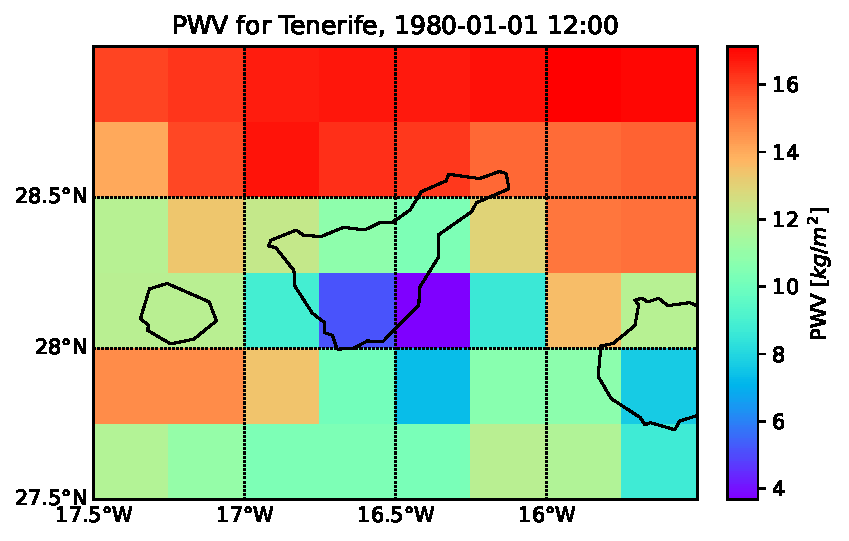
\includegraphics[width=1\textwidth]{PWV_Tenerife_1980-01-01_12-00_t}\end{tcolorbox}};%
\end{tikzpicture}%
}%
%
\end{frame}

\subsection{CDF .fits File and Seasonal Matrices}

\begin{frame}
\frametitle{CDFs \texttt{.fits} File}

\begin{columns}
\column{0.3\textwidth}

\onslide<1->{Statistical picture:}
\small
\begin{itemize}
\item<2-> Set of \alert{\textit{CDFs}} for every
          hour, month, \alert{relevant parameter}
\item<5-> $\sim$2MB \texttt{.fits} file
\end{itemize}%

\column{0.7\textwidth}
\onslide<3-5>{
\only<-5>{
\tikz\node at (1.7,-2) [fill=blue,shape=single arrow,text width=3cm,text height=2.5ex,overlay] {};

\begin{itemize}
\addtolength{\itemindent}{4cm}
\item TQL
\item TQI
\item \textcolor<4-5>{red}{PWV}
\item \textcolor<4-5>{red}{TS}
\item \textcolor<4-5>{red}{PS}
\item T10M
\item V10M
\item U10M
\end{itemize}
}%
}%
%
% Avoid spacing issue with images '%'
\includegraphics<6>[width=1.2\textheight]{PWV_Monthly_CDFs/PWV_Monthly_CDFs_Hour_0}%
\includegraphics<7>[width=1.2\textheight]{PWV_Monthly_CDFs/PWV_Monthly_CDFs_Hour_5}%
\includegraphics<8>[width=1.2\textheight]{PWV_Monthly_CDFs/PWV_Monthly_CDFs_Hour_11}%
\includegraphics<9>[width=1.2\textheight]{PWV_Monthly_CDFs/PWV_Monthly_CDFs_Hour_17}%
\includegraphics<10->[width=1.2\textheight]{PWV_Monthly_CDFs/PWV_Monthly_CDFs_Hour_23}%
%
\only<11>{%
\begin{tikzpicture}[remember picture,overlay]%
\node at (-6.5,2.9) {\begin{tcolorbox}[top=1pt, bottom=1pt, left=1pt, right=1pt, width=1.15\textwidth]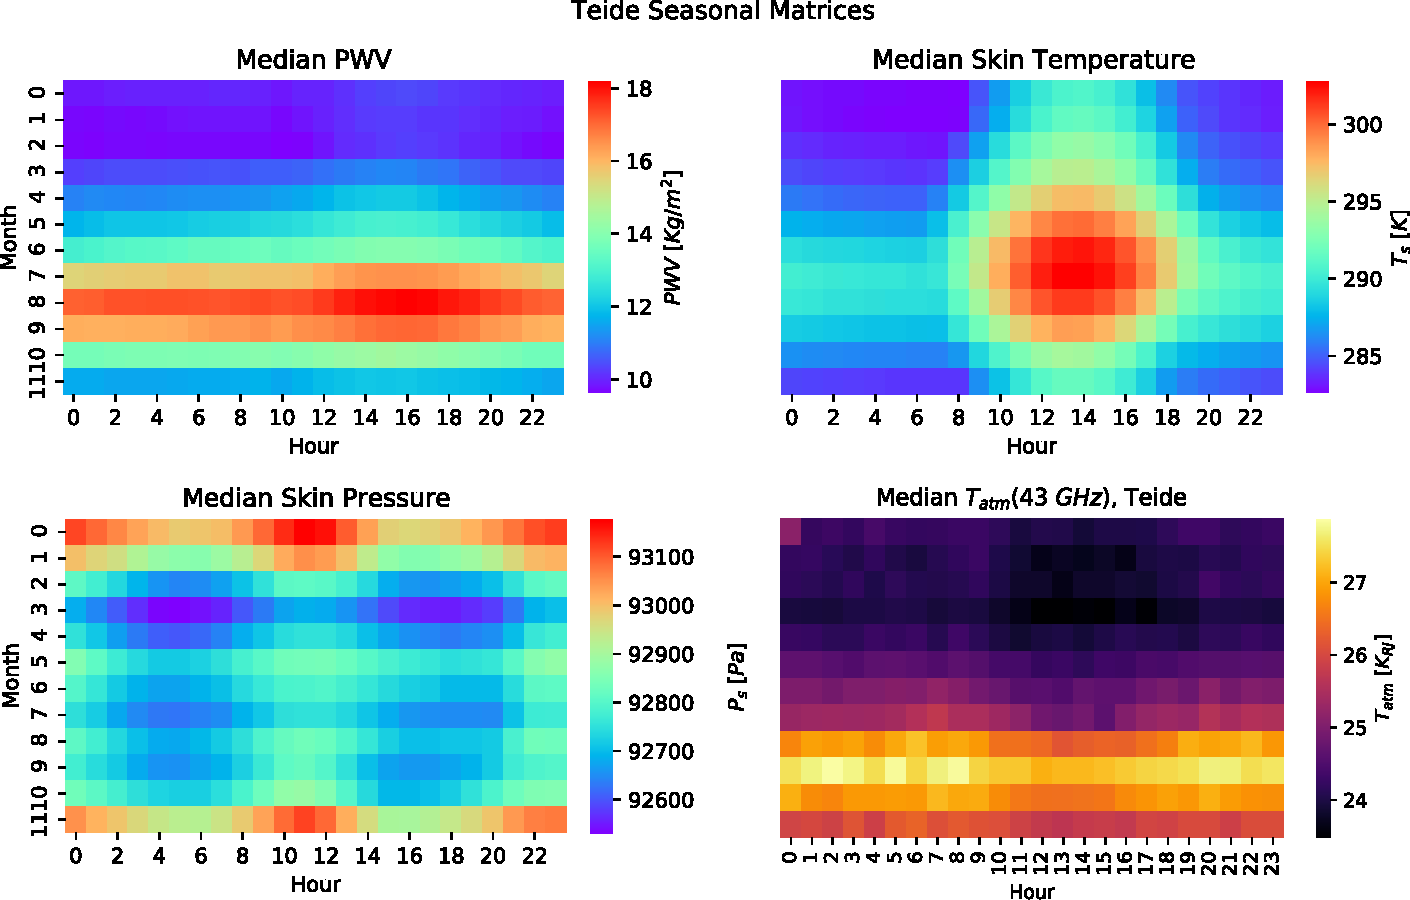
\includegraphics[width=1\textwidth]{Teide_Seasonal_Matrices+TATM}\end{tcolorbox}};%
\end{tikzpicture}%
}%
%
\end{columns}

\end{frame}

\section{Comparison with Measurements}

%\begin{frame}
%\frametitle{QUIJOTE-MFI Dataset \textcolor{red}{\small Forse questa slide \`e di
%troppo? Potrebbe bastare il primo grafico nella seguente + mio commento?}}
%
%\only<1-10>{
%QUIJOTE QT1 Telescope:
%\begin{itemize}
%\item<2-> \alert{Teide} Observatory
%\item<4-> Instituto de Astrofisica de Canarias
%\item<5-> \alert{MFI} (Multi Frequency Instrument) \onslide<6->{$\rightarrow$ Central frequencies
%          \alert{11}, \alert{13}, \alert{17}, \alert{19} GHz}
%\item<7-> $T_{atm}$ data from MFI \textit{sky dips}:
%
%\begin{itemize}
%\item<8-> \alert{444} points $\rightarrow$ December 2012-February 2015
%\item<9-> \alert{32} Channels
%\item<10-> \alert{Inhomogeneous time} distribution
%\end{itemize}
%
%\end{itemize}
%}
%
%\only<3>{
%\begin{tikzpicture}[remember picture,overlay]
%\node at (6.5,2) {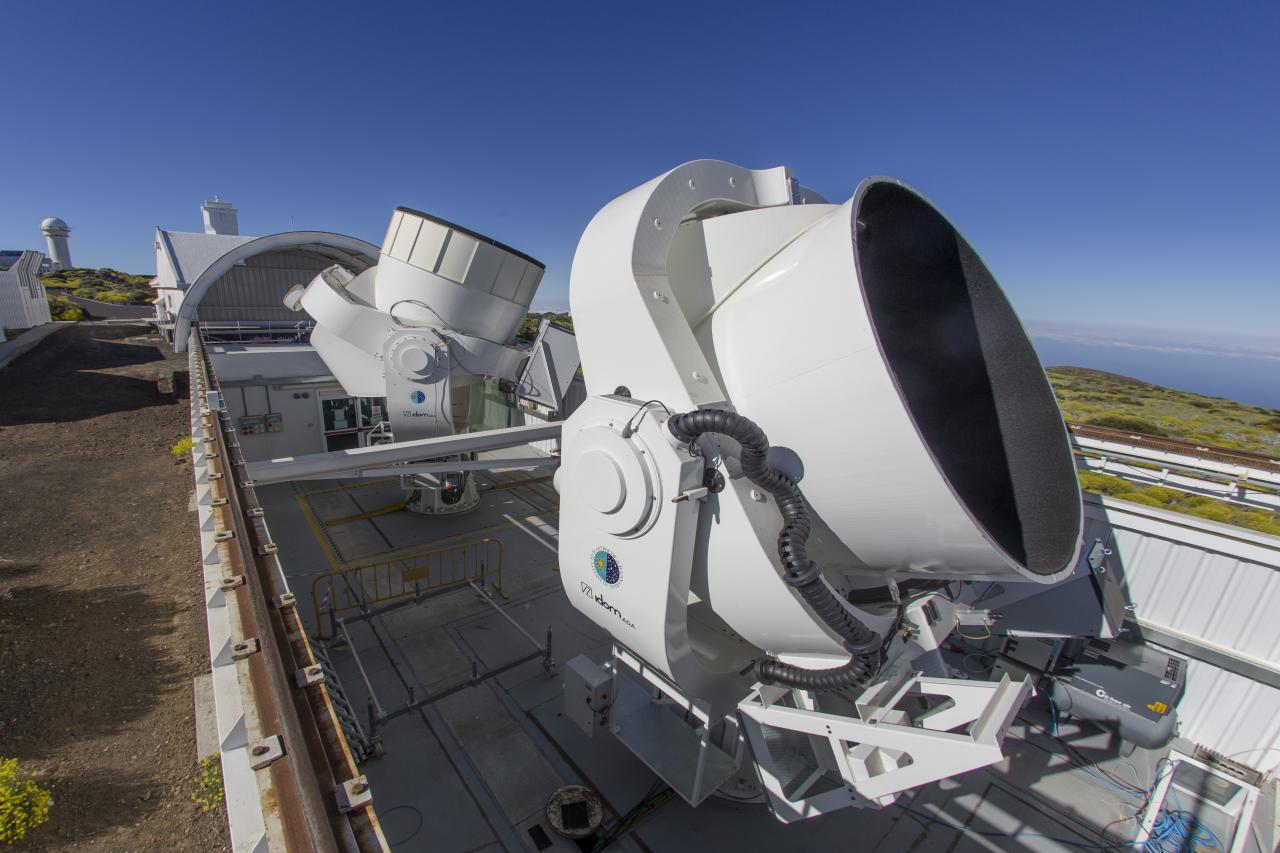
\includegraphics[width=0.75\textwidth]{QUIJOTE}};
%\end{tikzpicture}
%}
%
%\end{frame}

\subsection{Raw Simulation-QUIJOTE Data Comparison}

\begin{frame}
\frametitle{QUIJOTE-MFI Dataset \& Simulations}

\centering
\includegraphics<1>[width=0.75\textwidth]{QUIJOTE_Dataset_2}%
\includegraphics<2->[width=0.75\textwidth]{QUIJOTE-Sim}%
%
%\only<3->{%
%\tikzoverlay[text width=8cm] at (-8.8,4.3) {
%\begin{itemize}
%\item<3-> Simulation overestimates data
%\item<4-> Overestimation gets worse for higher frequencies
%\end{itemize}
%};
%}%

\end{frame}


\begin{frame}
\frametitle{ERA5 Spatial Resolution}

\centering
\includegraphics<1->[height=0.92\textheight]{PWV_Teide_1980-01-01_12-00}%
%
\only<2->{%
\tikz\draw[red,fill=red,overlay,remember picture] (-7.3,5.4) circle (1ex);%
}%
\only<3->{%
\tikz\node[yellow,overlay,remember picture,rotate=45] at (-6.8,3.8) {Low lands};%
}%
\only<4->{%
\tikz\node[yellow,overlay,remember picture] at (-4.5,2.3) {Ocean};%
}%

\end{frame}

\subsection{Calibration Strategy}

\begin{frame}
\frametitle{Calibration Coefficient}

\begin{columns}
        \begin{column}{0.28\textwidth}
                \alert{Balloon probe measurements} performed at Teide observatory:
                \begin{itemize}
                \item<2-> \alert{High spatial} resolution
                \item<3-> \alert{Low temporal} resolution $\rightarrow$ flight duration $\sim$ 12 hours
                \item<4-> \alert{One year} of data (2018)
                \end{itemize}
        \end{column}

        \begin{column}{0.68\textwidth}
        \onslide<5->{%
        \includegraphics<-7>[width=1\textwidth]{AM_CAL_Comparison}%
        \includegraphics<8>[width=1\textwidth]{Calibration_Coefficient}%
        \includegraphics<9>[width=1\textwidth]{Calibration_Coefficient_QUIJOTE}%
        }%
        \end{column}%
\end{columns}%
%
\only<6-7>{%
\tikzoverlay[text width=5cm] at (6.2,4.5) {%
\begin{block}{Calibration Coefficient}%
\begin{equation}%
k(\nu) = \frac{T_{sky}^\text{Probes}(\nu)}{T_{sky}^{CAL}(\nu)}%
\end{equation}%
\onslide<7>{Assumption: \textcolor{red}{not time dependent!}}%
\end{block}%
};%
}%
%
\end{frame}

\subsection{Calibrated Simulation-QUIJOTE Data Comparison}

\begin{frame}
\frametitle{QUIJOTE-MFI Dataset \& Calibrated Simulations}

\begin{columns}
        \begin{column}{0.59\textwidth}
        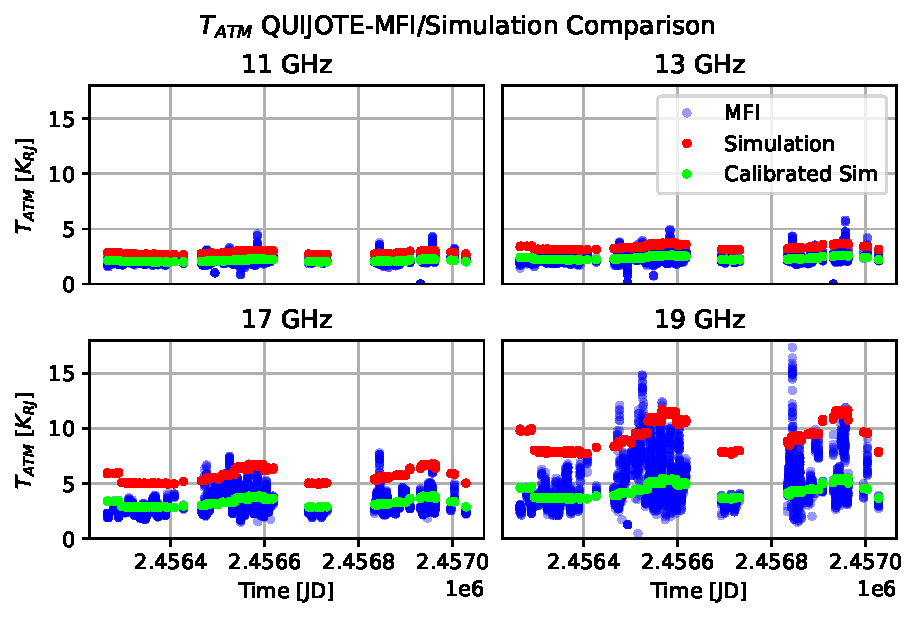
\includegraphics[width=1\textwidth]{QUIJOTE-Sim_calibrated}
        \end{column}
        \pause
        \begin{column}{0.39\textwidth}
        \vspace{0.5cm}
        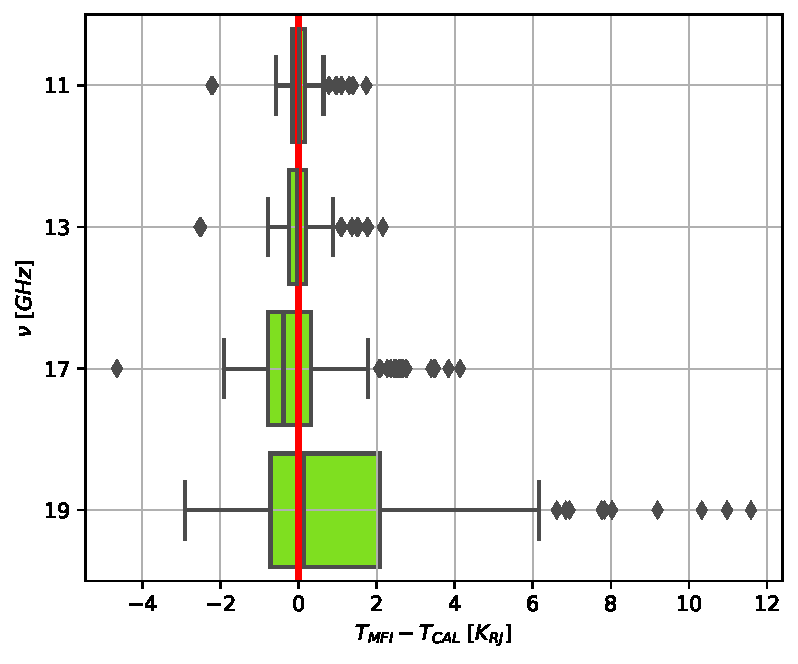
\includegraphics[width=1\textwidth]{QUIJOTE-Sim_calibrated_residuals_boxplot}
        \end{column}
\end{columns}

\end{frame}

\section{Conclusions}

\begin{frame}
\frametitle{Conclusions}

\begin{itemize}[<+->]
        \item \dots
        \item \dots
        \item \dots
\end{itemize}

\end{frame}

\end{document}
